\documentclass[xcolor=dvipsnames,aspectratio=169,9pt]{beamer}
\usefonttheme[onlymath]{serif}

\usepackage[T1]{fontenc}
\usepackage[utf8]{inputenc}
\usepackage[english]{babel}
\mode<presentation>
{
  \usetheme{default}
  \usecolortheme{default}
  \usefonttheme{default}
  \useinnertheme[shadow]{rounded}
  \useoutertheme{infolines}
% \setbeamertemplate{caption}[numbered]
}

\usepackage{graphicx}
\usepackage[percent]{overpic}
\usepackage[utf8]{inputenc}
\usepackage{array}
\usepackage{multirow}
\usepackage{amsmath}
\usepackage{xcolor}
\usepackage{csabamath}
\usepackage{animate}
\usepackage{listings}
\usepackage{svg}
\usepackage{multicol}
\usepackage{fontawesome}
\usepackage{lmodern}
\usepackage{textpos}
\usepackage[normalem]{ulem}

\usepackage[%
    backend=biber,
    bibencoding=utf8,
    texencoding=utf8,
    defernumbers=true,
    sorting=nyt,
    sortcites=true,
    block=none,
    indexing=false,
    citereset=none,
    isbn=true,
    url=false,
    doi=true,
    maxbibnames=99,
    style=alphabetic,
    %sorting=ynt
]{biblatex}
\addbibresource{references.bib}

\usepackage{changepage,threeparttable} % for wide tables

\usepackage{tcolorbox}

%\usepackage{enumitem}% http://ctan.org/pkg/enumitem

\frenchspacing
                
\makeatletter

    \setbeamertemplate{headline}
    {
    \leavevmode%
    \hbox{%
      \begin{beamercolorbox}[wd=\paperwidth,ht=2.24ex,dp=1ex,center]{section in head/foot}%
        \usebeamerfont{section in head/foot}\insertsectionhead\hspace*{2ex}-
        \usebeamerfont{subsection in head/foot}\hspace*{2ex}\insertsubsectionhead
      \end{beamercolorbox}%
    }%
    \vskip0pt%
    }
    \setbeamertemplate{headline}{}
    \setbeamertemplate{navigation symbols}{}
    \setbeamertemplate{frametitle}{%
    \nointerlineskip%
    \begin{beamercolorbox}[wd=\paperwidth,ht=2.0ex,dp=0.5ex, shadow=true]{frametitle}
        \hspace*{2ex}\insertframetitle
    \end{beamercolorbox}%
    }
  
  \definecolor{matlab_1}{rgb}{0.0000, 0.4470, 0.7410}
  \definecolor{matlab_2}{rgb}{0.8500, 0.3250, 0.0980}
  \definecolor{matlab_3}{rgb}{0.9290, 0.6940, 0.1250}
  \definecolor{matlab_4}{rgb}{0.4940, 0.1840, 0.5560}
  \definecolor{matlab_5}{rgb}{0.4660, 0.6740, 0.1880}
  \definecolor{matlab_6}{rgb}{0.3010, 0.7450, 0.9330}
  \definecolor{matlab_7}{rgb}{0.6350, 0.0780, 0.1840}
  
  \definecolor{CanvasBG}{RGB}{255,255,255}
  \definecolor{NormalTextCol}{RGB}{40,40,40}
  \definecolor{DisabledTextCol}{RGB}{100,100,100}

  \definecolor{BlockBG}{RGB}{235,235,235}
  \definecolor{BlockText}{RGB}{0,0,0}

\definecolor{FrameBG1}{RGB}{55,55,115} \definecolor{FrameText1}{RGB}{220,230,240}
\definecolor{FrameBG2}{RGB}{40,100,172}\definecolor{FrameText2}{RGB}{230,240,250}

  \definecolor{Red_bg}{RGB}{106,67,64}
  \definecolor{Text_on_red}{RGB}{255,236,234}
  
  \setbeamercolor{structure}{fg=NormalTextCol}
  \setbeamercolor{local structure}{fg=FrameBG2}
  \setbeamercolor{normal text}{fg=NormalTextCol, bg=CanvasBG}
  \setbeamercolor{example text}{fg=BlockText, bg=BlockBG}
  \setbeamercolor{alerted text}{fg=Text_on_red, bg=Red_bg}
  \setbeamercolor{titlelike}{fg=FrameText2, bg=FrameBG2}
  \setbeamercolor{block body}{fg=BlockText, bg=BlockBG}
  \setbeamercolor{block title}{fg=FrameText1, bg=FrameBG1}
  \setbeamercolor{palette primary}{fg = FrameText1,bg = FrameBG1}
  \setbeamercolor{palette secondary}{fg = FrameText2, bg = FrameBG2}
  \setbeamercolor{palette tertiary}{fg = FrameText1, bg = FrameBG1}
  \setbeamercolor{section in toc}{fg=NormalTextCol}
  \setbeamercolor{subsection in toc}{fg=DisabledTextCol}
  \setbeamertemplate{itemize items}[default]
  \setbeamertemplate{enumerate items}[default]
  \setbeamertemplate{subsection in toc}[unnumbered ball]
  \setbeamertemplate{section in toc}{%
	\leavevmode\leftskip=2.65ex%
 	\llap{\raisebox{0.19ex}{\textcolor{FrameBG2}{$\blacktriangledown$}}\kern1ex}%
  	\inserttocsection\par
  }

    %\logo{
\includegraphics[height=1cm]{elte_ik.png}}
    \newif\ifplacelogo % create a new conditional
    \placelogotrue % set it to true
    \logo{\ifplacelogo
\includegraphics[height=1cm]{images/elte_ik.png}\fi}
    \titlegraphic{\ifplacelogo
\includegraphics[height=1cm]{images/elte_ik.png}}
    \setbeamercolor{frametitle}{fg=white}

\renewcommand{\emph}[1]{\textcolor{FrameBG2}{\textbf{#1}}}

\makeatother

\newcommand{\nrw}[1]{\rvert_{_{#1}}}

\newcommand{\whitecolorbox}[1]{{\setlength{\fboxsep}{0pt}\colorbox{white}{#1}}}


\usepackage{listings}
\usepackage{color} %red, green, blue, yellow, cyan, magenta, black, white
\definecolor{mygreen}{RGB}{2,128,9}
\definecolor{mylilas}{RGB}{170,55,241}

\lstset{language=Matlab,%
    %basicstyle=\color{red},
    basicstyle=\tiny,
    breaklines=true,%
    morekeywords={matlab2tikz},
    keywordstyle=\color{blue},%
    morekeywords=[2]{1}, keywordstyle=[2]{\color{black}},
    identifierstyle=\color{black},%
    stringstyle=\color{mylilas},
    commentstyle=\color{mygreen},%
    showstringspaces=false,%without this there will be a symbol in the places where there is a space
    numbers=none,%
    numberstyle={\tiny \color{black}},% size of the numbers
    numbersep=9pt, % this defines how far the numbers are from the text
    emph=[1]{for,end,break},emphstyle=[1]\color{red}, %some words to emphasise
    escapeinside={(*@}{@*)} %to reference equations and figures
}
\def\ContinueLineNumber{\lstset{firstnumber=last}}
\def\StartLineAt#1{\lstset{firstnumber=#1}}
\let\numberLineAt\StartLineAt

\usepackage[displaymath, mathlines]{lineno}
\linenumbers

\title[SDF DNF]{\huge SDF-alapú CSG fák hatékony megjelenítése befoglaló dobozokkal}
%\subtitle{Subtitle}
\author{Gugi Gergely}
\institute[ELTE]{%
Eötvös Loránd Tudományegyetem

Shapr3d%
}    
\date[Shapr3D (03. Március 2026)]{%
}

%%%%%%%%%%%%%%%%%%% TITLE PAGE %%%%%%%%%%%%%%%%%%%%%
\makeatletter\setbeamertemplate{title page}{
\centering\vfill

\tcbox[colback=FrameBG1,colframe=white]{\centering\Huge
    \textcolor{FrameText1}{\inserttitle}
}\vfill

\if\empty\insertsubtitle
\else
\textit{\textbf{\textcolor{FrameBG2}{\Large
    \insertsubtitle
}}}\vfill    
\fi

\textit{\Large\insertauthor}\vfill

\insertinstitute\vfill

 \begin{tabular}{rl}\large
     Témavezető: & \large ~\textit{Bálint Csaba}, Ph.D.
 \end{tabular}\vfill


\includegraphics[height=1cm]{images/elte_fekvo_kek_logo.png}\hfill
\begin{minipage}[b][1cm][c]{.5\textwidth}\centering%
\large\insertdate
\end{minipage}\hfill

\includegraphics[height=1cm]{images/elte_ik.png}\vfill

}\makeatother
%%%%%%%%%%%%%%%%%%% END %%%%%%%%%%%%%%%%%%%%%

\definecolor{R0color}{RGB}{218,142,251}
\definecolor{R1color}{RGB}{ 77,182,215}
\definecolor{R2color}{RGB}{ 72,181, 69}
\definecolor{Dcolor}{RGB}{118,  0,226}

\setbeamercovered{%
  still covered={\opaqueness<1->{50}},
  again covered={\opaqueness<1->{30}}}


\begin{document} %D D D D D D D D D D D D D D D D D D D D D D D D D D D D

\frame[plain]{\titlepage}

% Orange theme
% \definecolor{FrameBG1}{RGB}{155,94,60}  \definecolor{FrameText1}{RGB}{255,200,160}
% \definecolor{FrameBG2}{RGB}{211,132,84} \definecolor{FrameText2}{RGB}{255,250,245}
% Purple theme
% \definecolor{FrameBG1}{RGB}{65, 47, 79}   \definecolor{FrameText1}{RGB}{229, 190, 236}
% \definecolor{FrameBG2}{RGB}{145, 127, 179}\definecolor{FrameText2}{RGB}{253, 226, 243}
% Teal-yellow theme
% \definecolor{FrameBG1}{RGB}{83, 113, 136} \definecolor{FrameText1}{RGB}{225, 212, 187}
% \definecolor{FrameBG2}{RGB}{200, 160, 110}\definecolor{FrameText2}{RGB}{238, 238, 238}
% Blue theme
% \definecolor{FrameBG1}{RGB}{55,55,115}\definecolor{FrameText1}{RGB}{220,230,240}
% \definecolor{FrameBG2}{RGB}{40,100,172}\definecolor{FrameText2}{RGB}{230,240,250}

\begin{frame}
\frametitle{Tartalom}
  %\begin{multicols}{2}
  \begin{columns}[onlytextwidth,T]
        \begin{column}{.45\textwidth}
            \tableofcontents
        \end{column}
        \begin{column}{0.45\textwidth}
        	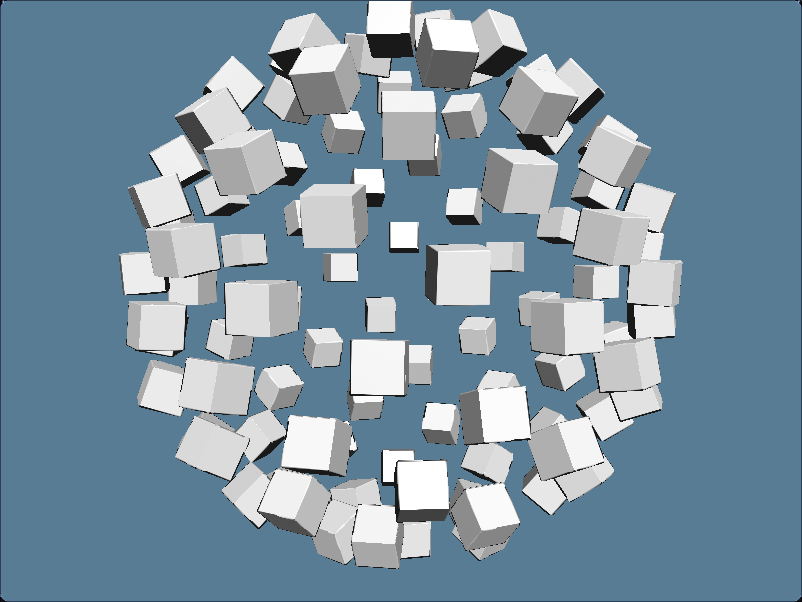
\includegraphics[width=\linewidth]{images/sdf_demo.png}
        \end{column}
    \end{columns}
  %\end{multicols}
\end{frame}

\section{Bevezető}
\subsection{SDF}
\begin{frame}{Mi az a távolságfüggvény (SDF)?}

\begin{columns}

\column{0.55\textwidth}
\begin{itemize}
    \item $f : \mathbb{R}^3 \to \mathbb{R}$

\item $
f(\mathbf{x}) =
\begin{cases}
    d(\mathbf{x}, \partial\Omega), & \mathbf{x} \notin \Omega \\
    0, & \mathbf{x} \in \partial\Omega \\
    -d(\mathbf{x}, \partial\Omega), & \mathbf{x} \in \Omega
\end{cases}
$
\end{itemize}

\column{0.45\textwidth}
\centering
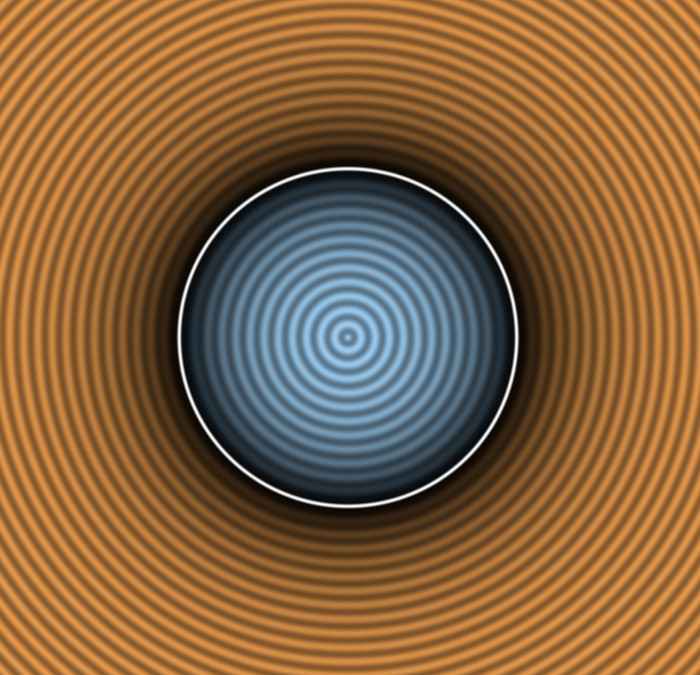
\includegraphics[width=\textwidth]{images/sdf_example.png}

\end{columns}
\end{frame}


\begin{frame}{Megjelenítési lehetőségek és kutatási irányok}

\begin{columns}

% pics
\column{0.55\textwidth}

\begin{itemize}

\uncover<1>\item \structure{Voxelizált reprezentáció}
\begin{itemize}
    \item<1> Előre kiértékelt SDF rácspontokon
    \item<1> Pontfelhőből rekonstruált távolságmező
\end{itemize}

\vspace{0.3cm}

\uncover<2>\item \structure{SDF rekonstrukció}
\begin{itemize}
    \item<2> Pontatlan vagy zajos mérésekből
    \item<2> Regularizáció és simítás
\end{itemize}

\vspace{0.3cm}

\uncover<3>\item \structure{Azonnali megjelenítés}
\begin{itemize}
    \item<3> Sphere tracing
    \begin{itemize}
            \item<3-> Csakis függvény alakban
    \end{itemize}
    \item<3> Iterációszám csökkentés
    \item<3> Adaptív lépésheurisztikák
\end{itemize}

\end{itemize}

%---------------- RIGHT COLUMN ----------------
\column{0.45\textwidth}

\only<1>{
    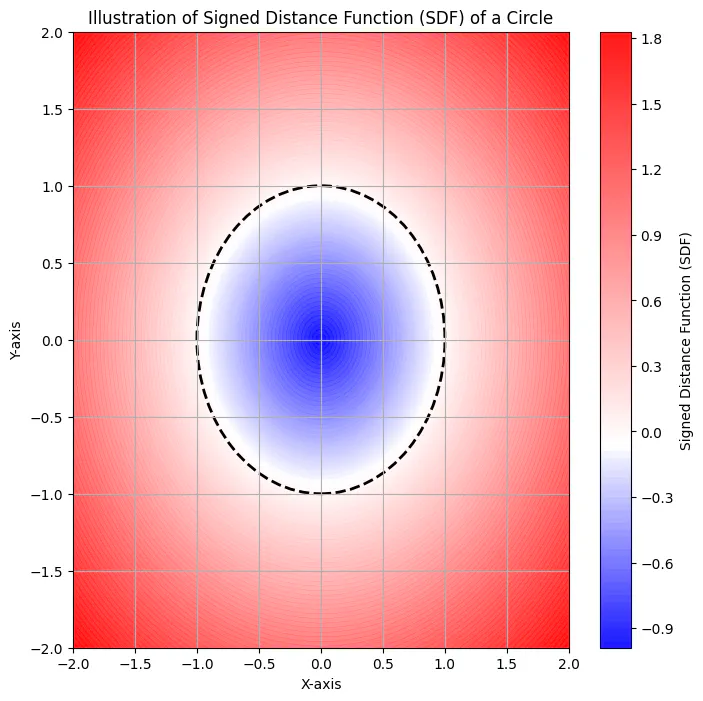
\includegraphics[width=\linewidth]{images/voxel_storage_sdf.png}
}

\only<2>{
    
\includegraphics[width=\linewidth]{images/sdf_fix.png}
}

\only<3>{
    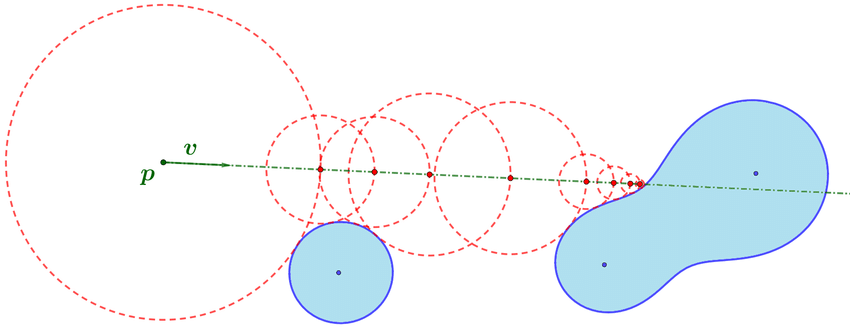
\includegraphics[width=\linewidth]{images/sphere_tracing_demo.png}
    %\cite{SphereTracingKep}
}

\end{columns}

\vspace{0.5cm}

\only<3>{
\textbf{A mi kutatásunk: hatékonyságnövelés az azonnali megjelenítésben.}
}

\end{frame}


\subsection{CSG}
%------------------------------------------------
\begin{frame}{SDF előállítása CSG fával}
\begin{columns}[T]
\begin{column}{0.45\textwidth}
Gyakori módszer: \textbf{CSG (Constructive Solid Geometry)}

\begin{itemize}
    \item Primitívek: gömb, doboz, henger, tórusz
    \item Halmazműveletek:
    \begin{itemize}
        \item Unió: $\min(f_1, f_2)$
        \item Metszet: $\max(f_1, f_2)$
        \item Különbség: $\max(f_1,-f_2)$
    \end{itemize}
\end{itemize}

Előny:
\begin{itemize}
    \item Átlátható
    \item Könnyen módosítható
\end{itemize}

Észrevételek:
\begin{itemize}
    \item Szükséges egy fordító CSG $\rightarrow$ SDF kód
    \item A generált kódból nehéz strukturális információt visszanyerni
\end{itemize}
\vfill
%Kép:\cite{CsikosBalazsKep}
\end{column}
\begin{column}{0.45\textwidth}


  
  \only<1>{
  
     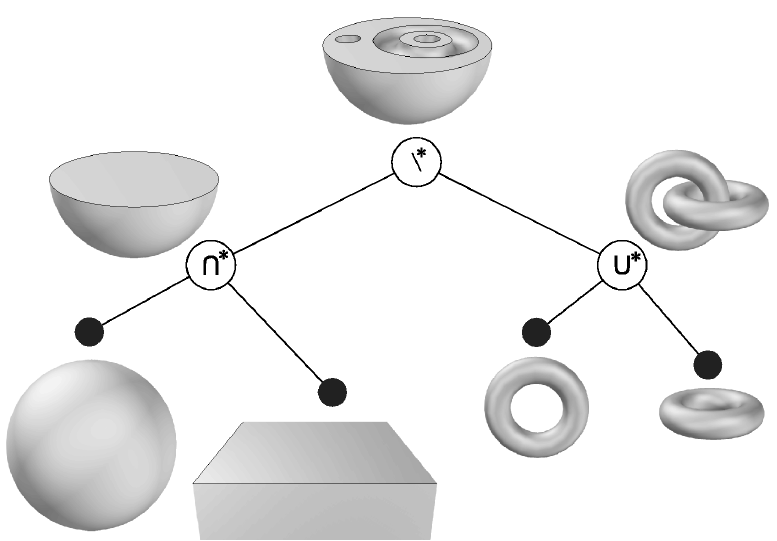
\includegraphics[width=\linewidth]{images/csikos_balazs_csg.png}
      
  }

  
  \only<2>{
    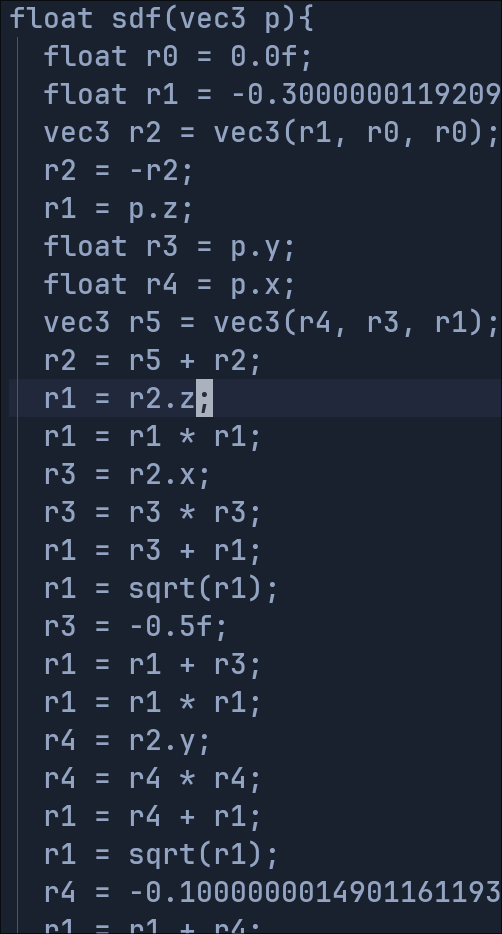
\includegraphics[height=0.8\paperheight]{images/csikos_balazs_sdf.png}

  }

\end{column}
\end{columns}
\end{frame}

%------------------------------------------------

\begin{frame}{A pontosság problémája}
\begin{columns}[T]
\begin{column}{0.45\textwidth}
Fontos megfigyelés:

Az unió és metszet műveletek:
\[
\min(f_1, f_2), \quad \max(f_1, f_2)
\]

\begin{itemize}
    \item Csak alsó becslés 
    \item Térben elkülöníthető testek távolságfüggvényei.
    \item Lassabb konvergencia sphere tracing során
\end{itemize}

\end{column}
\begin{column}{0.45\textwidth}


\includegraphics[width=\linewidth]{images/sdf_bad.png}
\end{column}
\end{columns}
\end{frame}

\section{Módszertan}
\subsection{Térbeli korlátozás}
%------------------------------------------------
\begin{frame}{Lokális térbeli korlátozás}
\begin{columns}[c]

\begin{column}{0.45\textwidth}


\textbf{Ne az egész térben értékeljük ki az SDF-et.}

Ha tudjuk, hogy az objektum csak egy adott dobozon belül létezik:

\begin{itemize}
    \item Csak ott érdemes sphere tracing-et végezni
    \item Csökken az iterációszám
    \item Gyorsabb konvergencia
\end{itemize}

Cél: \textbf{Automatikus befoglaló tér meghatározása}.
\vfill
\end{column}
\begin{column}{0.45\textwidth}
\only<1>{
\includegraphics[width=\linewidth]{images/sdf_bad.png}}
\only<2>{
\includegraphics[width=\linewidth]{images/sdf_bad_boxes.png}}
\only<4>{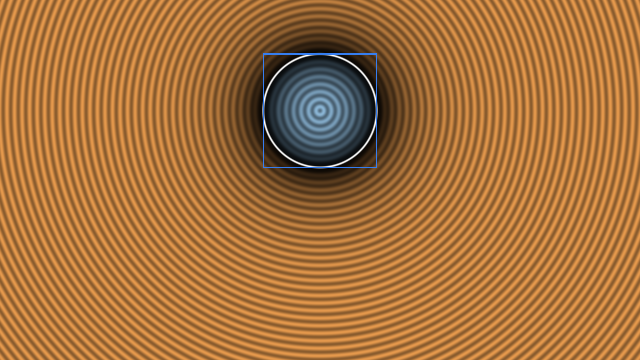
\includegraphics[width=\linewidth]{images/sdf_bad_only_sphere_sdf.png}}
\only<3>{
\includegraphics[width=\linewidth]{images/sdf_bad_only_box_sdf.png}}
\end{column}
\end{columns}
\end{frame}

%------------------------------------------------
\subsection{Reprezentáció}
\begin{frame}{Reprezentáció a CSG és a nyers SDF között}

\begin{columns}[c]
\begin{column}{0.45\textwidth}
	\only<1>{
		\centering
		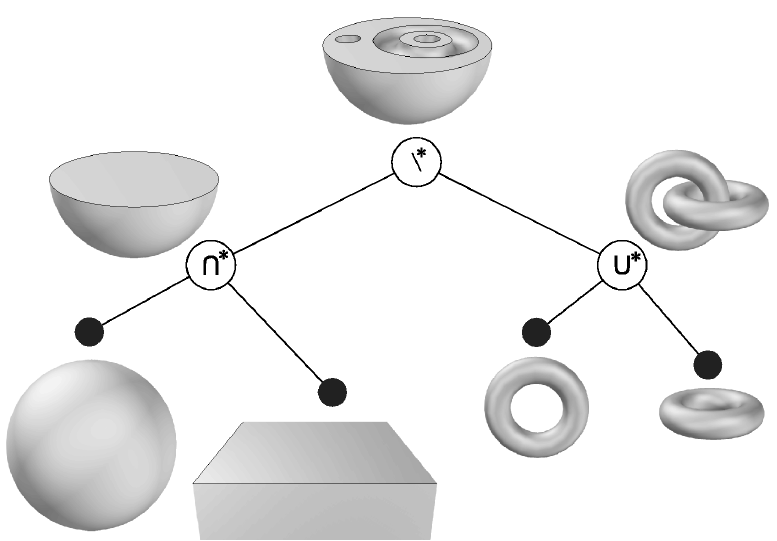
\includegraphics[width=\linewidth]{images/csikos_balazs_csg.png}
		
	}
	\only<2>{
		
		\centering
		
		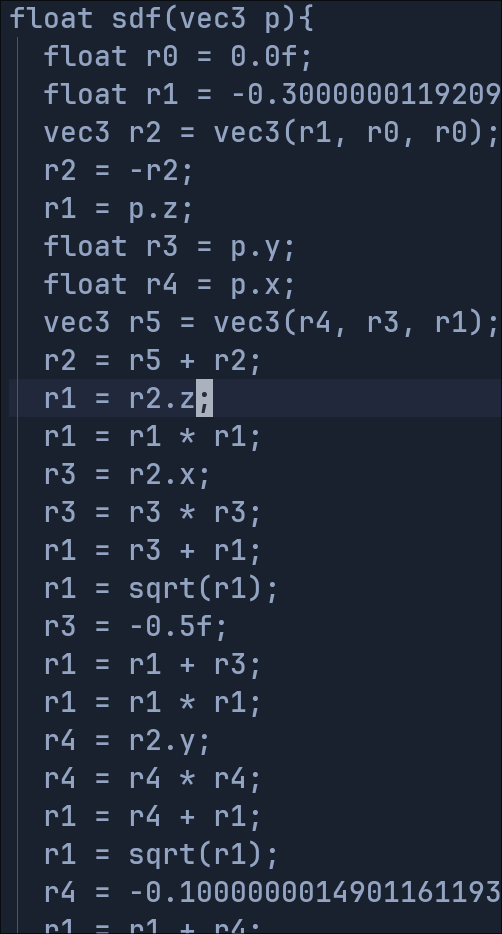
\includegraphics[height=0.8\paperheight]{images/csikos_balazs_sdf.png}%
		
	}
	\only<3>{
		\centering
		
		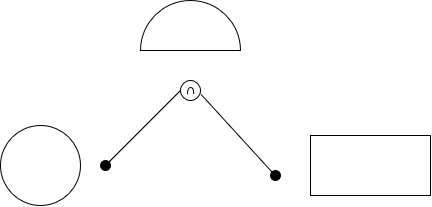
\includegraphics[width=\linewidth]{images/stored_csg_1.png}
	}
	\only<4>{
		\centering
		
		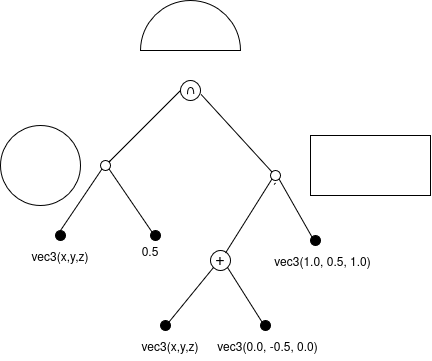
\includegraphics[width=\linewidth]{images/stored_csg_2.png}
	}
\end{column}
\begin{column}{0.45\textwidth}
A tiszta CSG túl korlátozott.  
A tiszta generált SDF túl alacsony szintű.

Megoldásunk:
\begin{itemize}
    \item Egy köztes reprezentáció
    \item A kiértékelési fa részben absztrakt
    \item Bizonyos műveletek precízen tárolva
\end{itemize}

Cél:
\begin{itemize}
    \item Struktúra megőrzése
\end{itemize}
\end{column}


\end{columns}
\end{frame}

%------------------------------------------------
\subsection{Intervallum aritmetika}
\begin{frame}{Intervallum aritmetika}

\begin{columns}[c]

\begin{column}{0.45\textwidth}
\only<1>{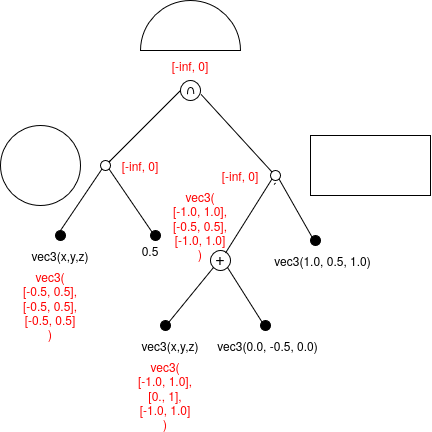
\includegraphics[width=\linewidth]{images/intervallum_back.png}}
\only<2>{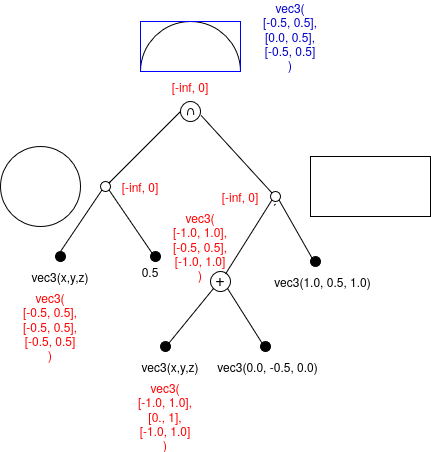
\includegraphics[width=\linewidth]{images/intervallum_back_solved.png}}
\end{column}
\begin{column}{0.45\textwidth}
	Kérdés: hol negatív a függvény?
	
	Megoldás:
	\begin{itemize}
		\item Intervallum aritmetikával visszakövetjük
		\item Nehezebb mint a sdf-értéket meghatározni egy adott térrégión belül.
	\end{itemize}
	
	Tulajdonságok:
	\begin{itemize}
		\item Konzervatív
		\item Gyors(abb és megbízhatóbb mint LP)
	\end{itemize}
	Miért kell absztrakt fa?
	\begin{itemize}
		\item Doboz vs Gömb.
	\end{itemize}
	
\end{column}
\end{columns}
\end{frame}


%------------------------------------------------
\subsection{Lineáris egyenletrendszer}
\begin{frame}{Félterek kezelése}
\begin{columns}[c]

\begin{column}{0.45\textwidth}
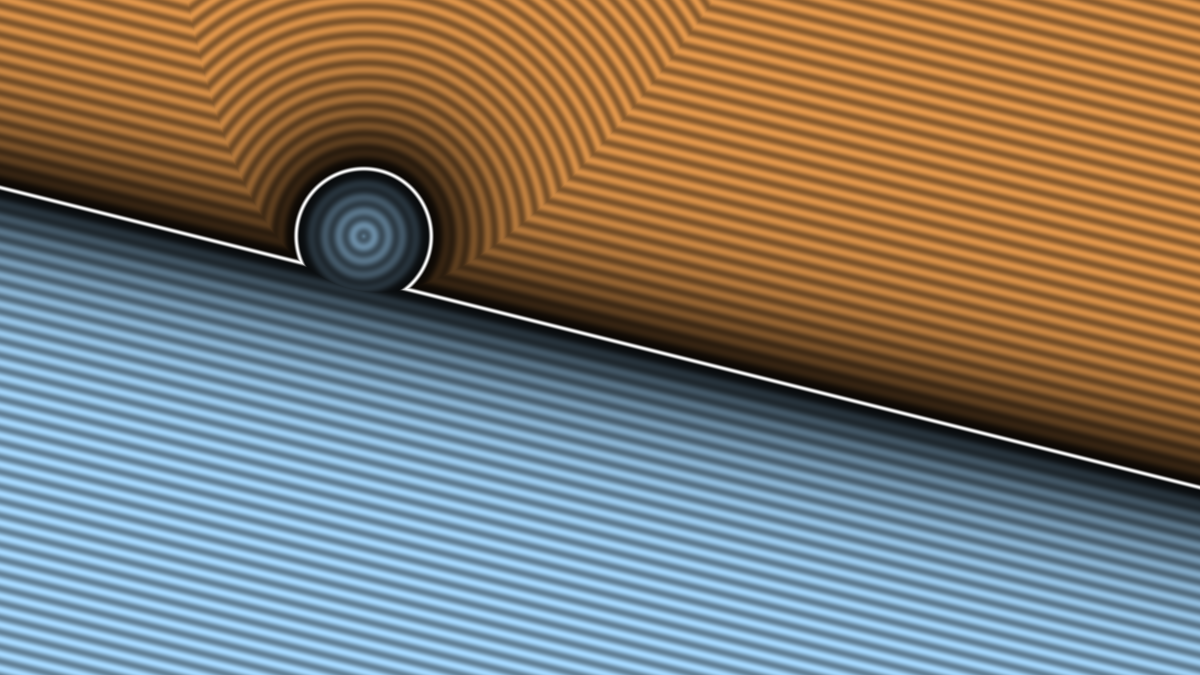
\includegraphics[width=\linewidth]{images/half_space.png}
\end{column}
\begin{column}{0.45\textwidth}
	
	Probléma:
	\begin{itemize}
		\item Félterek végtelen kiterjedésűek
	\end{itemize}
	
	Megoldás:
	\textbf{Félterek metszeteként *is* tároljuk a befoglaló teret.}
	
	\[
	dot(\mathbf{n},\mathbf{x}) + d \le 0
	\]
	
	A befoglaló poliéder:
	\[\begin{cases}
			dot(\mathbf{n_1}, \mathbf{x}) + d_1 <=0\\
			dot(\mathbf{n_2}, \mathbf{x}) + d_2 <=0\\
			...\\
			dot(\mathbf{n_k}, \mathbf{x}) + d_k <=0\\
		\end{cases}\]
	
	
	
	
	Előny:
	\begin{itemize}
		\item Végtelen objektumok kezelhetők
		\item Affin transzformációk pontos kezelése
		\item Forgatás nem torzítja túl a becslést
	\end{itemize}
	
\end{column}
\end{columns}
\end{frame}

%------------------------------------------------

\begin{frame}{Mit nyerünk ezzel?}

\begin{columns}[T]
\begin{column}{0.45\textwidth}
A módszer lehetővé teszi:

\begin{itemize}
    \item Szűk befoglaló doboz számítását
    \item $f(\mathbf{x})\leq m$ pontok halmazának lekérdezése
    \item Részfák prune-olását
\end{itemize}

Diszjunktív normálforma(DNF):
\begin{itemize}
    \item Egyszerűbb uniók
    \item Korai elágazás-elimináció

\end{itemize}
\begin{align*}
	A \cap (B \cup C) &= (A \cap B) \cup (A \cap C) \\
	\overline{A \cap B} &= \overline{A} \cup \overline{B}
\end{align*}


\end{column}
\begin{column}{0.45\textwidth}
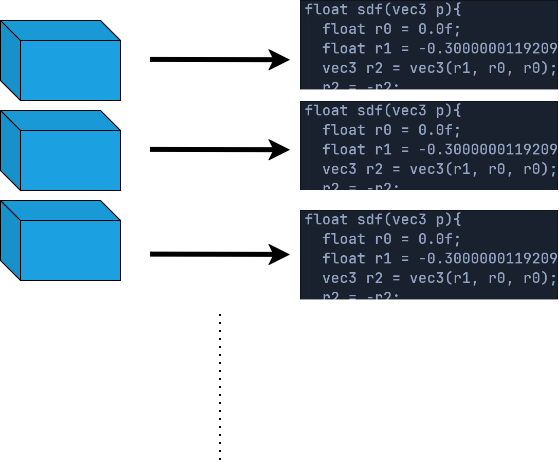
\includegraphics[width=\linewidth]{images/opt/DNF.png}
\end{column}
\end{columns}

\end{frame}
\begin{frame}
	\centering
	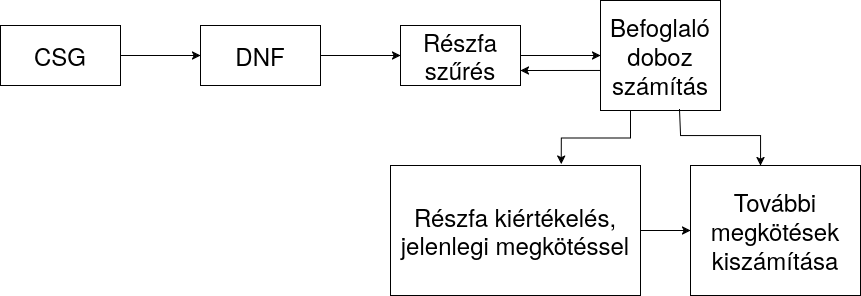
\includegraphics[width=0.8\linewidth]{images/intervallum_pipeline.png}
\end{frame}

%------------------------------------------------
\section{Megjelenítés}

\begin{frame}{Pipeline bontás és teljesítmény}
\begin{columns}[T]
\begin{column}{0.45\textwidth}
	Egy sdf:
\begin{itemize}
	\item Mindent visszafonunk
	\item Ez referenciaként szolgál a méréshez.
\end{itemize}



Ha minden kis doboz külön pipeline-t kap:

\begin{itemize}
    \item Üres terekben verhetetlen.
    \item Sok doboz esetén pipeline váltási költség nő
\end{itemize}



%Az unió műveletek helyettesíthetők:

%Előny:
%\begin{itemize}
	%\item Elkerülhető a problémás $\min$ művelet
	%\item Tiszta propagáció
	%\item Stabilabb sphere tracing
%\end{itemize}
\end{column}
\begin{column}{0.45\textwidth}
	\only<2>{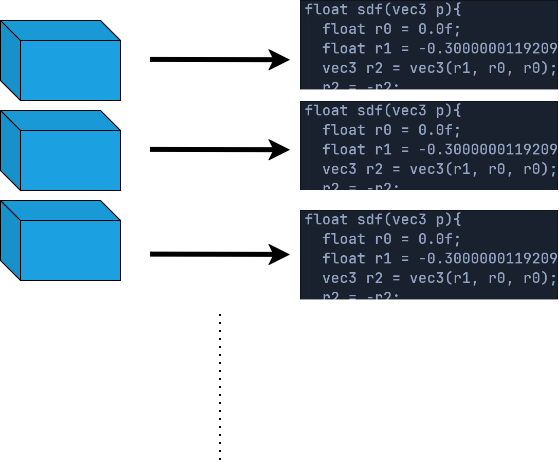
\includegraphics[width=\linewidth]{images/opt/DNF.png}}
	\only<1>{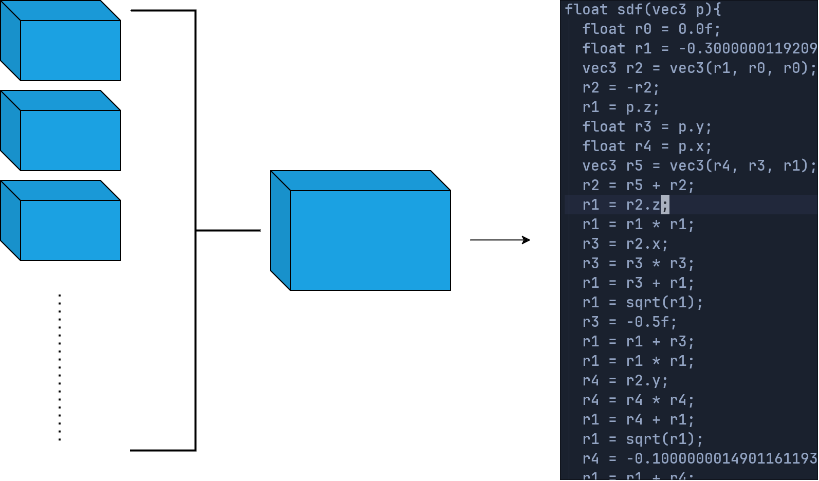
\includegraphics[width=\linewidth]{images/opt/NO_DNF.png}}
\end{column}
\end{columns}
\end{frame}

\begin{frame}
	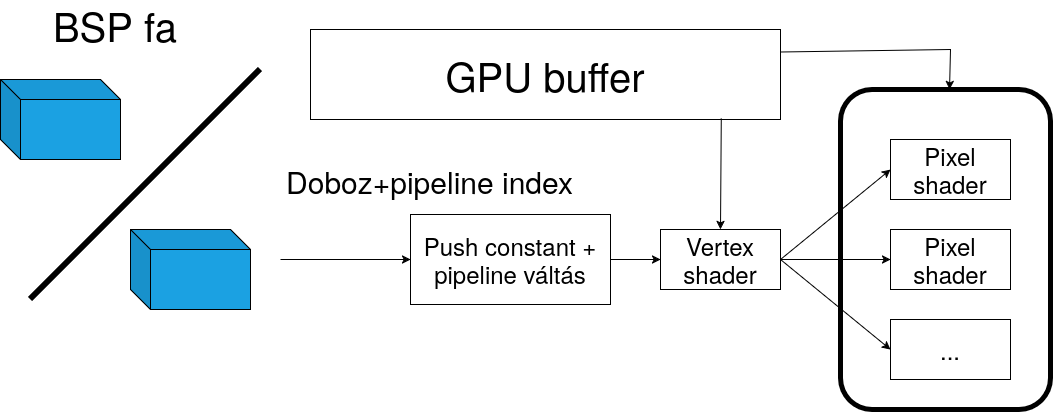
\includegraphics[width=\linewidth]{images/pipeline.png}

\end{frame}

%------------------------------------------------
\begin{frame}{Részfák összevonása}
\begin{columns}[T]
\begin{column}{0.45\textwidth}
Megfigyelés:

\begin{itemize}
    \item Sok részfa csak konstansban különbözik
    \item Térben ismétlődő objektumok
\end{itemize}

Lehetséges optimalizáció:
\begin{itemize}
    \item Azonos struktúrák összevonása
    \item Paraméterek GPU memóriából
    \item Pipeline váltások csökkentése
\end{itemize}

Probléma:
\begin{itemize}
    \item Térbeli összefüggés szükséges
    \item Nem lokális dobozok összevonása nem hoz nyereséget
\end{itemize}
\end{column}
\begin{column}{0.45\textwidth}
	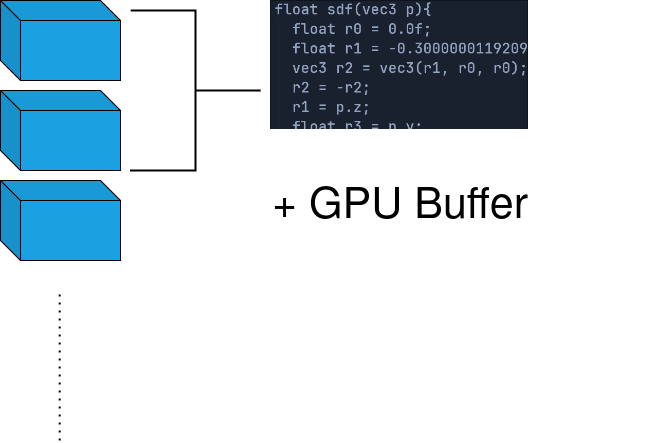
\includegraphics[width=\linewidth]{images/opt/DNF_const_merge.png}
\end{column}
\end{columns}
\end{frame}
\begin{frame}[fragile]{Részfa elimináció}
	\begin{columns}[c]
		\begin{column}{0.45\textwidth}
			Megfigyelés:
			\begin{itemize}
				\item A részfák határai találkoznak (pl. unió műveleteknél).
				\vspace{0.5cm}
					\item \texttt{min()} művelet $\Rightarrow$ \texttt{select} utasítás.
					\item Döntés a részfa indexe alapján.
			\end{itemize}
		\end{column}
\begin{column}{0.5\textwidth}
	\begin{lstlisting}[language=C++, basicstyle=\ttfamily\small]
		// Eredeti
		float dist =  min(d1, d2);
		
		// Helyett
		float dist = 
		(pipeline_ind == 1) ?
			  d1 : d2;
	\end{lstlisting}
\end{column}
	\end{columns}
\end{frame}

\begin{frame}{Összefoglaló}
	\begin{itemize}
		\item SDF
		\item Naiv
		\item Monolitikus
		\item Indexelt
		\item Instanced
		\item Parametrikus
	\end{itemize}
\end{frame}
\begin{frame}{Eredmények}

	Ide még jönnek a képek.
			
		\begin{table}[htbp]
			\centering
			\begin{tabular}{|l|c|c|c|c|c|c|}
				\hline
				\textbf{Scene $\mu$s} & \textbf{SDF} & \textbf{Naiv} & \textbf{Monolitikus} & \textbf{Indexelt} & \textbf{Instanced} & \textbf{Parametrikus} \\ \hline
				pipe & 920 & 725 & 889 & 850 & 796 & ! \\ \hline
				miniature high & 1215 & 231 & 1205 & 1889 & 1200 & 485 \\ \hline
				miniature low & 1180 & 260 & 385 & 1789 & 1236 & 595 \\ \hline
				miniature head-on & 1460 & 366 & 566 & 2450 & 1350 & 660 \\ \hline
				DH & 1460 & 185 & 408 & 49300 & 36910 & 660 \\ \hline
				DH 2.7k obj & FAIL 0.6 s & 800 & FAIL 608 & - & - & - \\ \hline
				2500 boxes & FAIL & 792 & - & - & - & - \\ \hline
				1000 boxes & 232200 & 2200 & & & & \\ \hline
			\end{tabular}
			
			\caption{GPU: 2080 SUPER}
			\label{tab:timing_data}
		\end{table}
\end{frame}

	%------------------------------------------------
\begin{frame}{Összefoglalás}
\begin{columns}[T]
\begin{column}{0.45\textwidth}
Bemutatott módszer:

\begin{itemize}
    \item Köztes reprezentáció CSG és nyers SDF között
    \item Intervallum aritmetika + féltér metszetek
    \item Szűk befoglaló tér meghatározása
    \item Részfa alapú optimalizáció
    \item Pipeline váltások csökkentése
\end{itemize}
\vfill
\centering
\Huge \emph{Köszönöm a figyelmet!}

\end{column}
\begin{column}{0.45\textwidth}
\end{column}
\end{columns}
\end{frame}

\end{document}